\chapter{波动方程}
\intro{本章讨论波动方程的建立、达朗贝尔公式和波动的基本性质。}

\section{弦振动方程的建立}

\begin{theorem}[弦振动方程]
长度为 $L$ 的理想弹性弦的横向振动：
\[
\frac{\partial^2 u}{\partial t^2}=a^2\frac{\partial^2 u}{\partial x^2}
\]
其中 $a=\sqrt{T/\rho}$，$T$ 为张力，$\rho$ 为线密度。
\end{theorem}

\section{达朗贝尔公式}

\begin{mydefinition}{达朗贝尔公式}
初值问题
\[
\begin{cases}
u_{tt}=a^2 u_{xx},&-\infty<x<+\infty,\;t>0\\
u(x,0)=\phi(x),\quad u_t(x,0)=\psi(x)
\end{cases}
\]
的解为：
\[
u(x,t)=\frac{1}{2}[\phi(x+at)+\phi(x-at)]+\frac{1}{2a}\int_{x-at}^{x+at}\psi(s)\,ds
\]
\end{mydefinition}

\begin{proof}
利用变量替换 $\xi=x+at$，$\eta=x-at$，将方程化为 $u_{\xi\eta}=0$，积分两次即得。
\end{proof}

\begin{figure}[htbp]
\centering
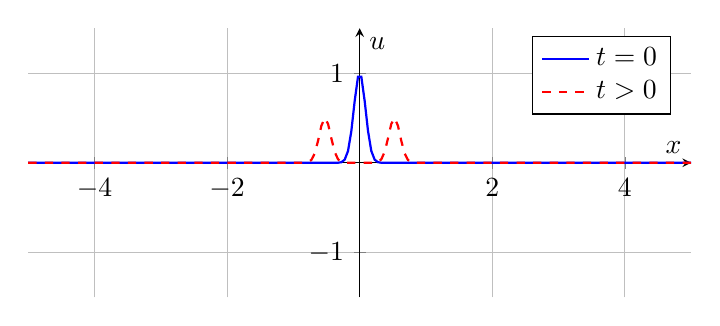
\begin{tikzpicture}
\begin{axis}[
	axis lines=middle,
	xlabel=$x$,
	ylabel={$u$},
	xmin=-5,xmax=5,
	ymin=-1.5,ymax=1.5,
	legend pos=north east,
	grid=major,
	width=10cm,height=5cm,
]
\addplot[blue,thick,domain=-5:5,samples=200]{exp(-deg(x)^2/50)};
\addplot[red,dashed,thick,domain=-5:5,samples=200]{0.5*(exp(-(deg(x)-30)^2/50)+exp(-(deg(x)+30)^2/50))};
\legend{$t=0$,$t>0$}
\end{axis}
\end{tikzpicture}
\caption{波动传播}
\end{figure}

\section{波动的性质}

\begin{proposition}[传播速度]
解以速度 $a$ 向左右两个方向传播，不改变波形。
\end{proposition}

\begin{proposition}[能量守恒]
\[
E(t)=\frac{1}{2}\int_0^L\left(\rho u_t^2+Tu_x^2\right)dx=\text{const}
\]
\end{proposition}

\begin{remark}
当 $\psi=0$ 时，初始波形 $\phi(x)$ 分裂为两个半幅波，分别向左右传播。
\end{remark}
